\section{Back-test results}

The implementation of back-test results is based on running the portfolio revision model for each month until the last portfolio revision at 2014-06-18.
The portfolio revision model is performed for each month, where $x^\up{old}_{i}$ is updated every run, with the previous portfolio concerning the historical month return of the current month.

The optimal portfolio mix for each period considering all its revision for both risk averse and risk neutral strategies are illustrated in Figure~\ref{fig:tradingportfolios}.
The risk averse strategy always obtain a mixed portfolio in order to minimize the risk of bad return.
One can verify that the IAU assets is in general the base of the portfolio mix for risk averse strategy. On the other hand, in the early times FXI asset has high participation, since that ETF has an upward tendency until the crash. After the crash, IAU has a very good upward tendency.
At this point IBB start slowly a upward tendency, which is more steeper in later periods.
In this way and based on the behaviour of the ETFs in Figure~\ref{fig:prices_selected}, the portfolio revision obtained for both perspectives is as expected.

In the $1/N$ strategy, on the first trading day we invest  an equal amount into each asset, and then leave the assets be for the entire trading period.

Since we are investing into 10 assets at a cost of 0.1\% of the trading volume, it costs us 1000 DKK to make the initial trade.
The remaining 999.000 DKK are left to grow during the entire period.

This strategy yields an annualized return of 5.7\% for the max-mean assets, and of 2.4\% for the min-stdev.

\begin{figure}[tp]
\centering
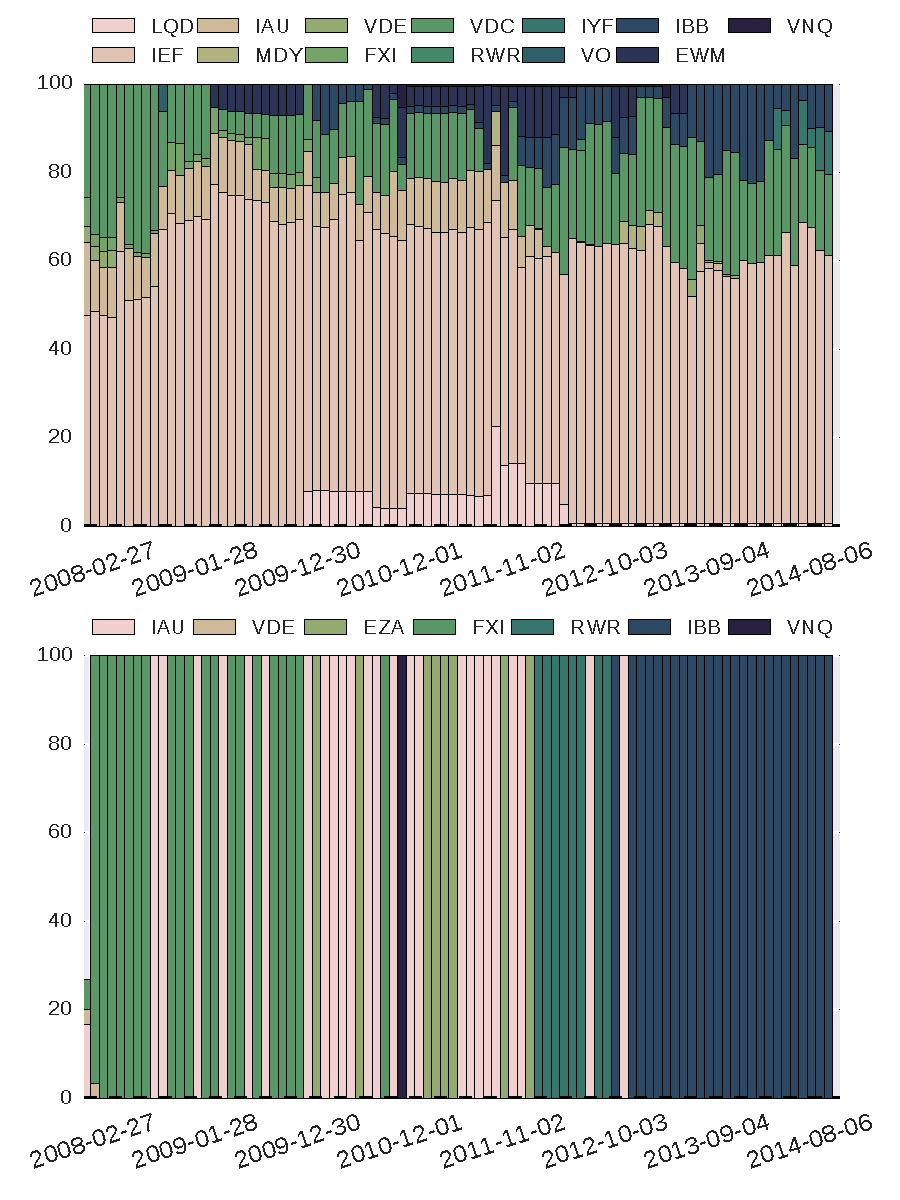
\includegraphics{../pic/trading_portfolio.pdf}
\caption{Portfolios found by the risk-averse (top) and risk-neutral (bottom) trading strategies.}
\label{fig:tradingportfolios}
\end{figure}

The portfolio value over the time for each of the strategies is presented in Figure~\ref{fig:tradingforecastedvalues}.
One can see that different strategies has different average behaviours, as well as the worst and best case of the scenarios.
The risk neutral strategy is the strategy that get higher return in the end of the period of investment. 
However, it does not mean that is the best strategy among all periods.
On average, the ideal strategy throughout the time is the use of both strategies to maximize the expected return.
In the early six months is advised the use of risk neutral strategy.
Than risk averse should be used until the early months of 2013.
In the remaining months, risk neutral ensures more return to the investor.

\begin{figure}[tp]
\centering
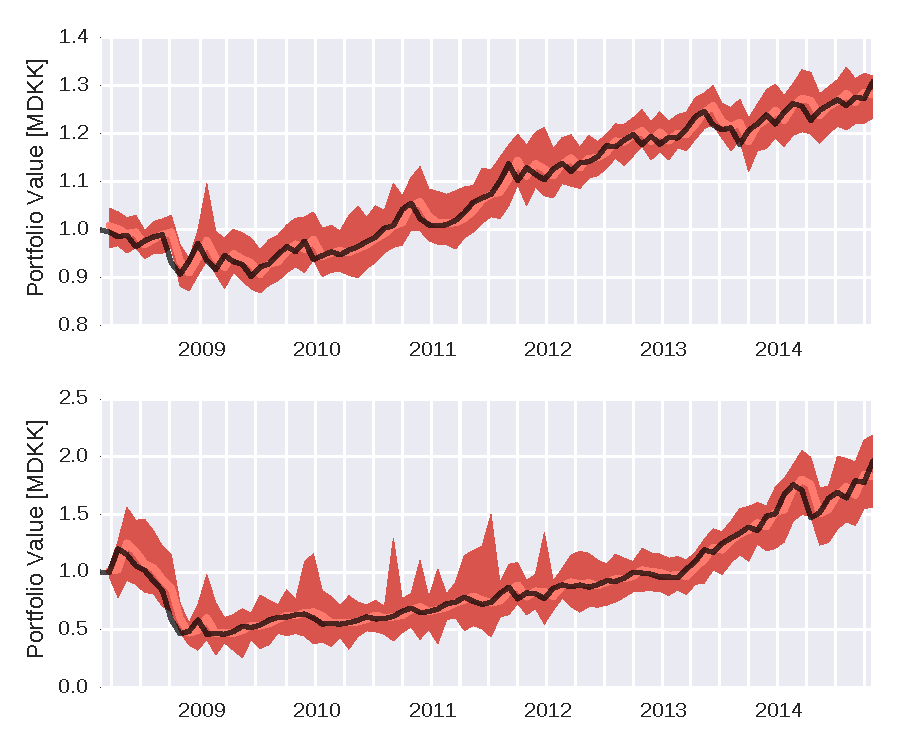
\includegraphics{../pic/trading_forecasted_value.pdf}
\caption{Nominal values of portfolios over time (Black line) versus forecasted mean value (light red). The shaded region indicates the maximum and minimum forecasted values of the ensembles. The risk avers (top) and risk neutral (bottom) strategies for portfolio valueare considered.}
\label{fig:tradingforecastedvalues}
\end{figure}

Regarding the results of portfolio revision model considering the scenario generation of moment matching, we conclude that the patterns of the results are very similar.

In order to compare a 1/N strategy with the strategy results of risk averse and risk neutral is presented the Figure~\ref{fig:tradingportfoliovalues}.
Furthermore, is considered the results of each strategy (risk averse and risk neutral) for each scenario generation method (bootstrap and moment matching).

\begin{figure}[tp]
\centering
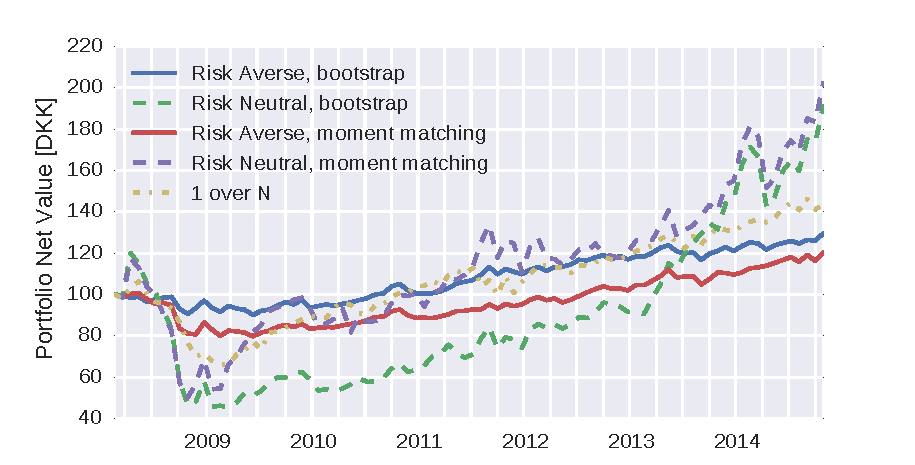
\includegraphics{../pic/trading_portfolio_value.pdf}
\caption{Net values of portfolios over time. (Net value = nominal value minus cumulative trading costs)}
\label{fig:tradingportfoliovalues}
\end{figure}

One can see that the risk averse strategy from the bootstrap method present on average higher portfolio value than the same strategy but based on moment matching method.
On the other hand, risk neutral strategy from moment matching strategy presents on average higher portfolio values than the strategy based on bootstrap method.
Regarding to the 1/N strategy, one can identify that is a strategy that returns a stable portfolio value throughout the periods.
However, is a strategy that presents results between the two extreme strategies (risk averse and risk neutral).
In the end, is expected a higher return value on risk averse strategy, and the lower return value on risk neutral strategy.

A comparison between the trading strategies considering different ways of evaluate the strategies is shown in Table~\ref{tbl:strategytabel}.

\begin{table}[tpbh]
\caption{Comparison of trading strategies}\label{tbl:strategytabel}
\centering
\begin{tabular}{lrrrl}
\toprule
{} & Final Nominal &  Trading &  Final Net & Annualized \\
{} & Value & Costs & Profit & Return \\
\midrule
Risk Averse, bootstrap        &              1259714 &          10810 &            248904 &             3.6 \% \\
Risk Neutral, bootstrap       &              1639882 &          43283 &            596599 &             7.7 \% \\
Risk Averse, moment matching  &              1172530 &           5797 &            166733 &             2.5 \% \\
Risk Neutral, moment matching &              1701345 &           8787 &            692558 &             8.7 \% \\
1 over N                      &              1462676 &              0 &            462676 &             6.2 \% \\
\bottomrule
\end{tabular}

\end{table}

It is noteworthy that the trading costs among the strategies from bootstrap method present higher value than the strategies based on moment matching method.
In respect to scenario generation based on bootstrap method, the trading costs of risk neutral strategy is higher than risk averse strategy. 
In a approximated way, the trading cost is sensible the quadruple.
Regarding the trading costs of both strategies based on moment matching model, is clearly that risk neutral strategy is about 50\% higher than risk averse strategy.
 
